\chapter{Trees}
\label{chp: trees}
In this chapter are introduced the fundamentals concepts of tree as abstract data type, and the most used algorithms related to trees \cite{wikitrees} (\href{https://en.wikipedia.org/wiki/Tree_(data_structure)}{Trees, Wikipedia}).

\section{General Definitions}
A \textbf{tree} is an abstract datatype that simulate a hierarchical structure. A tree is a particular kind of a linked list where there are more next elements. The base element of a tree is called \textbf{node} while the first element is called \textbf{root}.

\begin{figure}[H]
	\begin{center}
		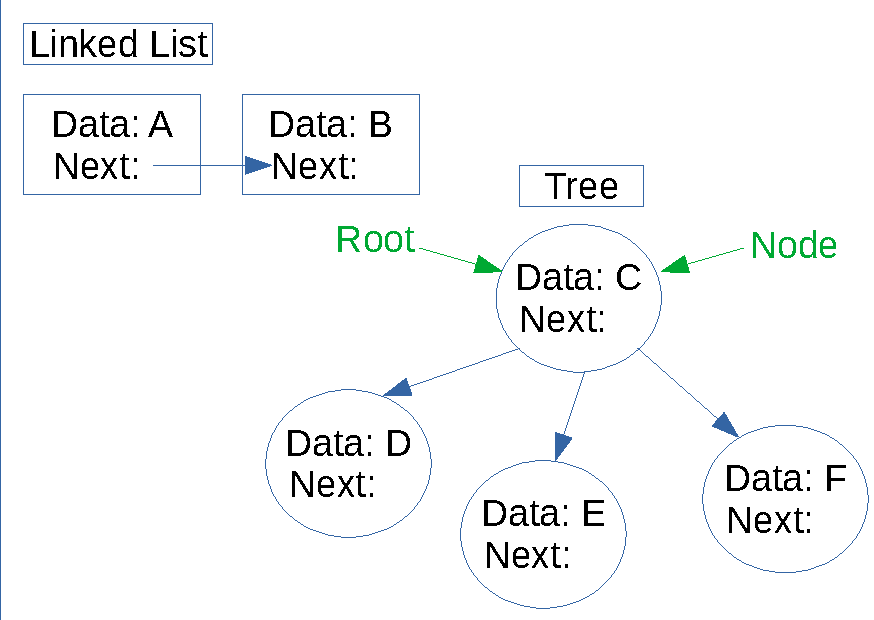
\includegraphics[scale=.6]{chapters/trees/images/trees_1.pdf}
		\caption[Elements of a tree and linked list]{Elements of a tree and linked list}
		\label{trees_1}
	\end{center}
\end{figure}

Trees must be completed connected structures, this means that there are not any nodes which are not connected to anything (Figure \ref{trees_2} case (a)), and there must not be present any cycles (Figure \ref{trees_2} case (c)).

\begin{figure}[H]
	\begin{center}
		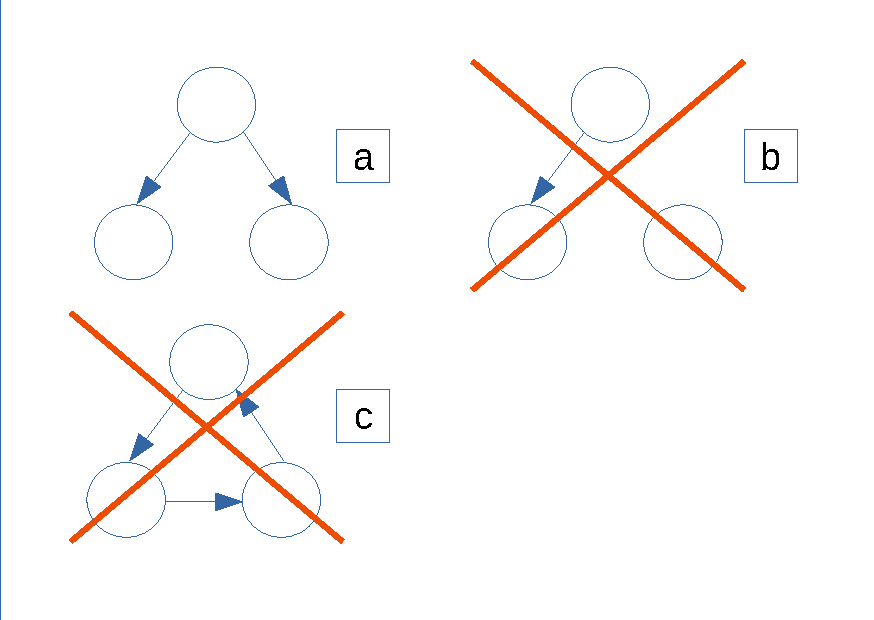
\includegraphics[scale=.6]{chapters/trees/images/trees_2.pdf}
		\caption[Possible structures of a tree]{Completed connected structure (a), a non completed connected structure (b), and a cycle (c)}
		\label{trees_2}
	\end{center}
\end{figure}

Trees are a hierarchical structures divided into layers: the first layer is the one belonging to the root node, the first node of a tree. The next element of the root are called children, which became parents in case they have next node connected as well. The last nodes of a trees are the nodes which do not have any children and they are called \textbf{leaf}. The numbers of connections is called \textbf{height}. A set of connections creates a \textbf{path}. The numbers of edges starting from the root to a node is called \textbf{depth}.
All this definitions are defined in following figure (Figure \ref{trees_3}).

\begin{figure}[H]
	\begin{center}
		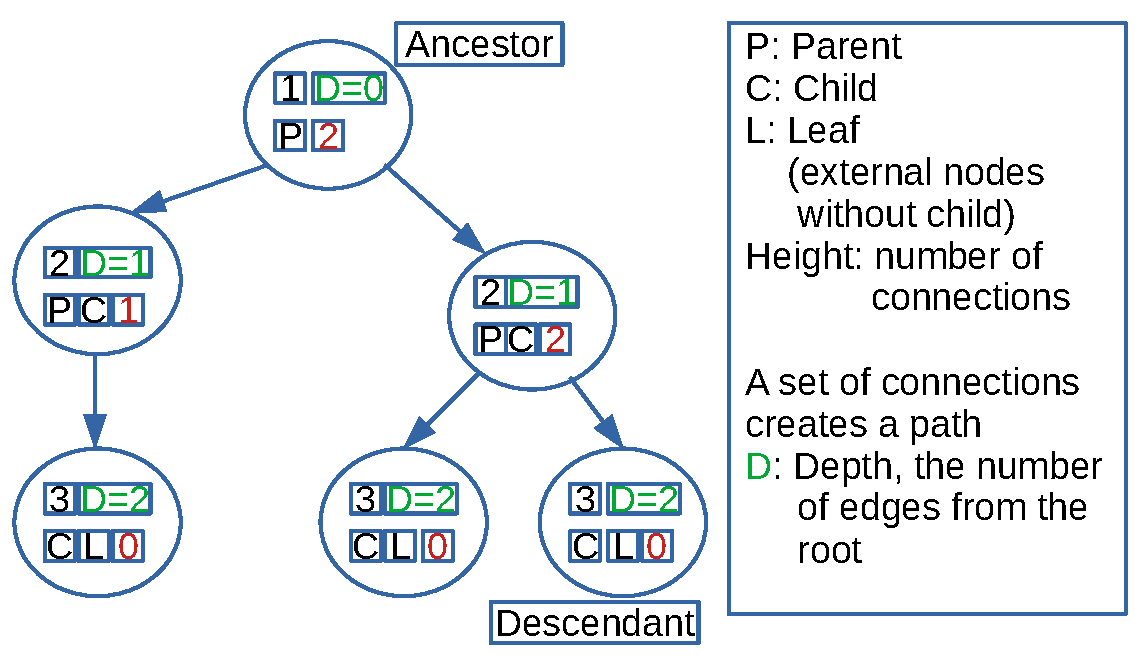
\includegraphics[scale=.6]{chapters/trees/images/trees_3.pdf}
		\caption[A tree and its fundamentals elements]{A tree and its fundamentals elements}
		\label{trees_3}
	\end{center}
\end{figure}

\section{Tree Traversal}
Which way is the most efficient for visiting all the nodes of a tree? Is it more efficient looking layer by layer or looking at subtrees? There are two different ways to traverse a tree: the \textbf{depth-first search} (\textbf{DFS}) and the \textbf{breath-first search} (\textbf{BFS}). In the first one the priority is to look at the children of a node, instead in the second one the priority is to look at the node of the same layer \ref{trees_4}.

\begin{figure}[H]
	\begin{center}
		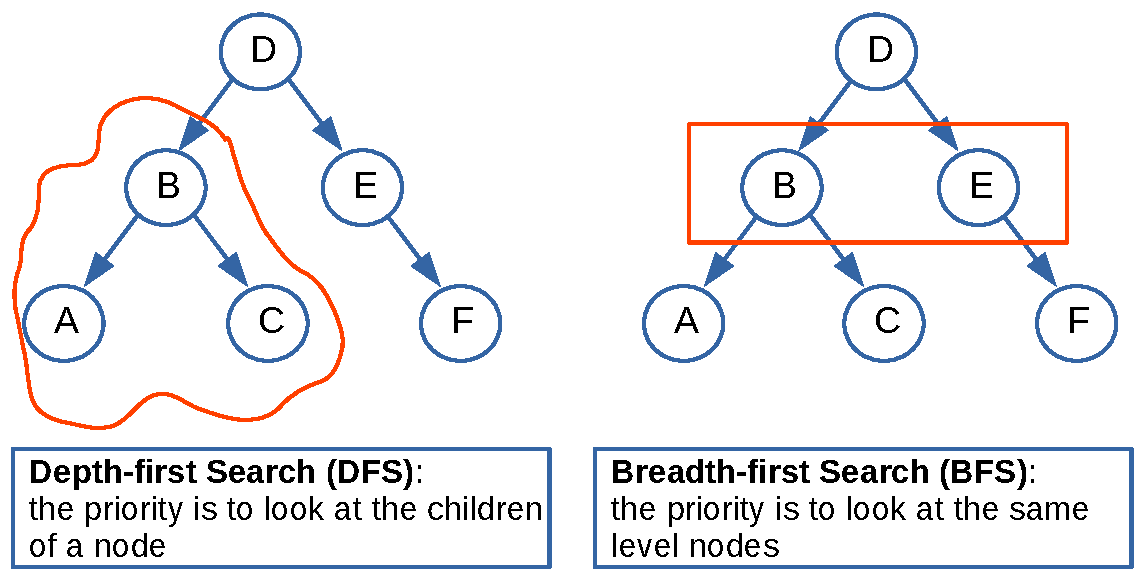
\includegraphics[scale=.6]{chapters/trees/images/trees_4.pdf}
		\caption[The depth-first search and the breath-first search]{The depth-first search and the breath-first search}
		\label{trees_4}
	\end{center}
\end{figure}

\subsection{Depth-first search}
In the depth-first search there are several different ways to perform a search on a tree.
\paragraph{Pre-order search}
In the \textbf{pre-order search} the first node to be checked as visited is the root. The following node is the left child by convention. Once checked the left child the process is repeated until the first node without any children is reached. At that point the same process is applied to the right side: all the nodes on the right are checked until all the nodes are checked as visited \ref{trees_5}.

\begin{figure}[H]
	\begin{center}
		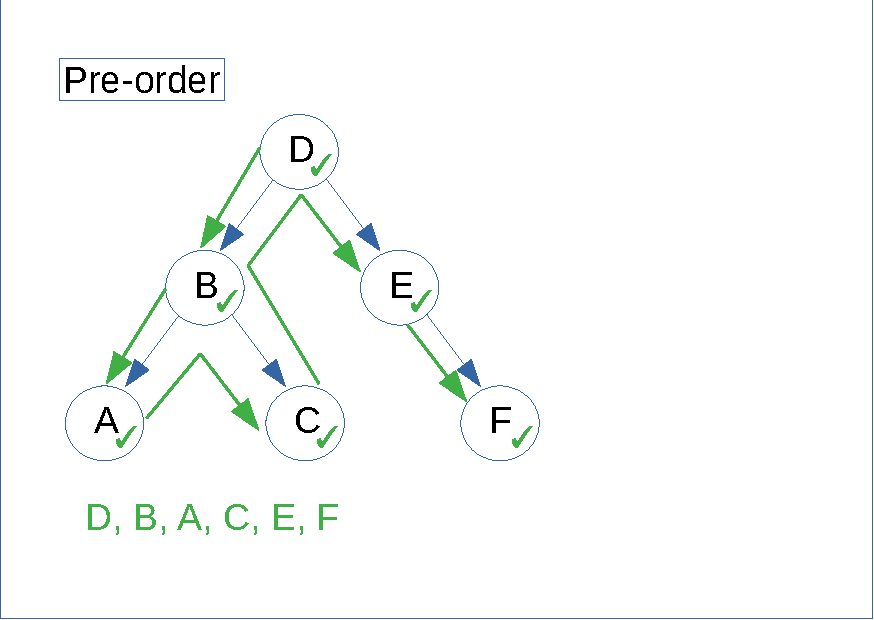
\includegraphics[scale=.6]{chapters/trees/images/trees_5.pdf}
		\caption[Pre-order search]{Pre-order search}
		\label{trees_5}
	\end{center}
\end{figure}

\paragraph{In-order search}
In the \textbf{in-order search} the first node to be checked is the first node without children on the left side. Once checked off this node the next one to be checked off is its parent, and the process is repeated again on the right side of the nodes, until all the nodes are checked off.

\begin{figure}[H]
	\begin{center}
		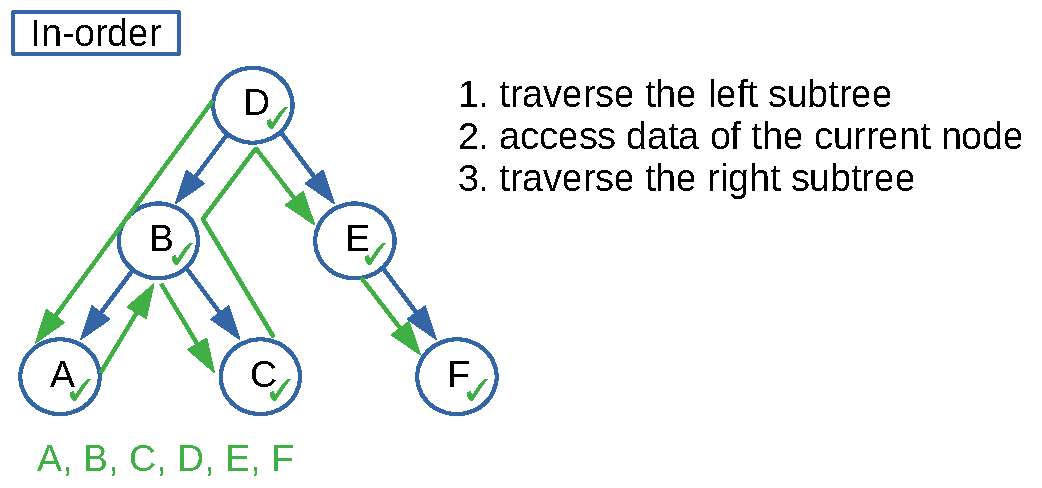
\includegraphics[scale=.6]{chapters/trees/images/trees_6.pdf}
		\caption[In-order search]{In-order search}
		\label{trees_6}
	\end{center}
\end{figure}

\paragraph{Post-order search}
In the \textbf{post-order search} the first node to be checked off is the first node without children on the left side. Once checked off this node the next one to be checked off is the one which does not have any children. Once all the nodes of the current left subtree without any children are checked off, the parents can be checked off, and the whole process is repeated until all the nodes are checked off.

\begin{figure}[H]
	\begin{center}
		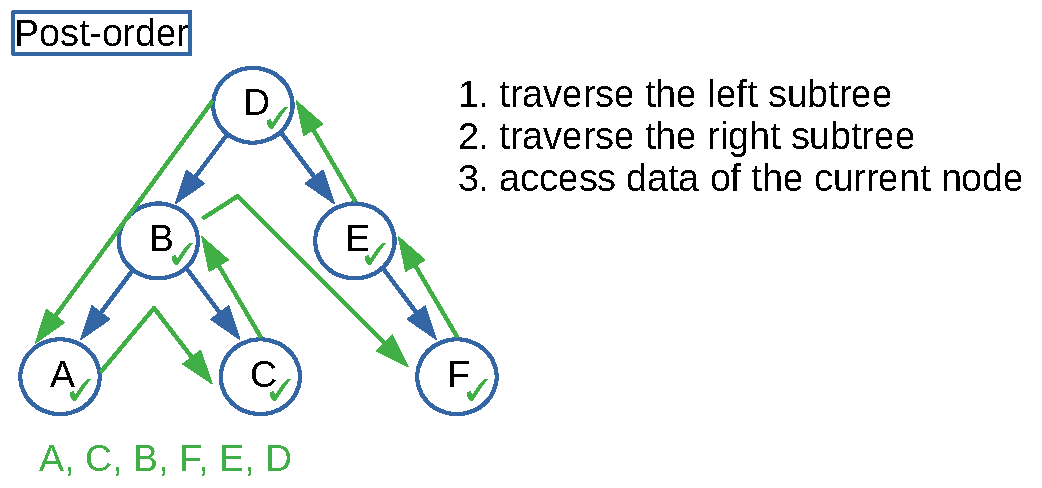
\includegraphics[scale=.6]{chapters/trees/images/trees_7.pdf}
		\caption[Post-order search]{Post-order search}
		\label{trees_7}
	\end{center}
\end{figure}

\section{Binary Trees}
\textbf{Binary trees} are trees in which the parent has at most two children (0, 1, 2 are the only number of admitted children). On binary trees some operations like searching, deleting, and inserting can be easily and efficiently done. 
\subsection{Search}
To search an element in the tree one of the previous methods can be used. Because in a general tree there is no ordering this means that potentially all the elements of the tree can be visited, then the complexity results in \(O(n)\).

\begin{figure}[H]
	\begin{center}
		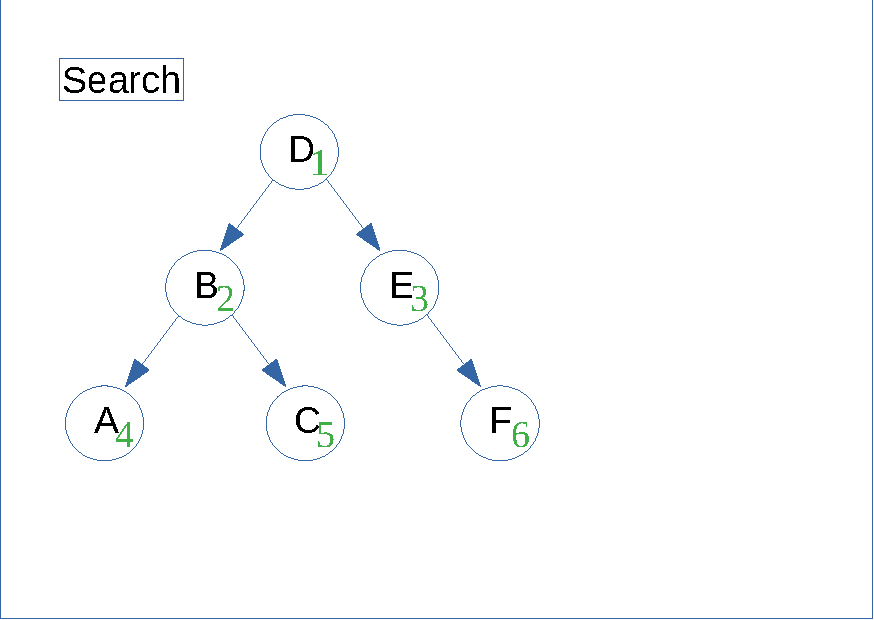
\includegraphics[scale=.6]{chapters/trees/images/trees_8.pdf}
		\caption[Search on a tree]{Search on a tree}
		\label{trees_8}
	\end{center}
\end{figure}

\subsection{Delete}
Before the delete process there is always a search one for finding the element to be deleted. If the element to be deleted is a leaf, deleting it is not a problem because there are not any children to be moved. Instead if the node to be removed has some children there are several opportunities to reorganize the nodes, because the condition for a binary tree must remain valid (a node can have at most two nodes). So there are several strategies. Let us consider the following tree \ref{trees_9}. 
\begin{itemize}
\item If the node to be removed has only one child it can be replaced by the child node (case 1 \ref{trees_9}).
\item If the node to be removed has two children it can be replaced with the child node which has no children node (case 2 \ref{trees_9}).
\item If the node to be removed has two children which have again children as well, in this case there are several options which can be done. For example on child node can be moved to the position of the one to be removed (case 3 \ref{trees_9}).
\end{itemize} 

\begin{figure}[H]
	\begin{center}
		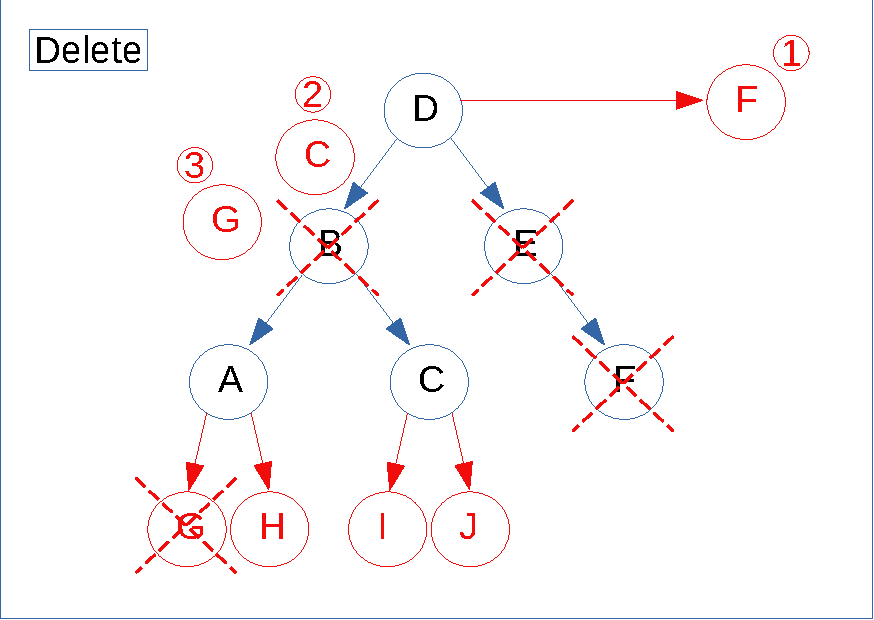
\includegraphics[scale=.6]{chapters/trees/images/trees_9.pdf}
		\caption[Delete an element of a tree]{Delete an element of a tree}
		\label{trees_9}
	\end{center}
\end{figure}

\subsection{Insert}
Insert a new element to a binary tree is not a hard operation, because it is enough to find a node which can take a new children node. In the worst case to find the proper node in which a child can be add the farthest leaf must be reached (case 1 \ref{trees_10}).

\begin{figure}[H]
	\begin{center}
		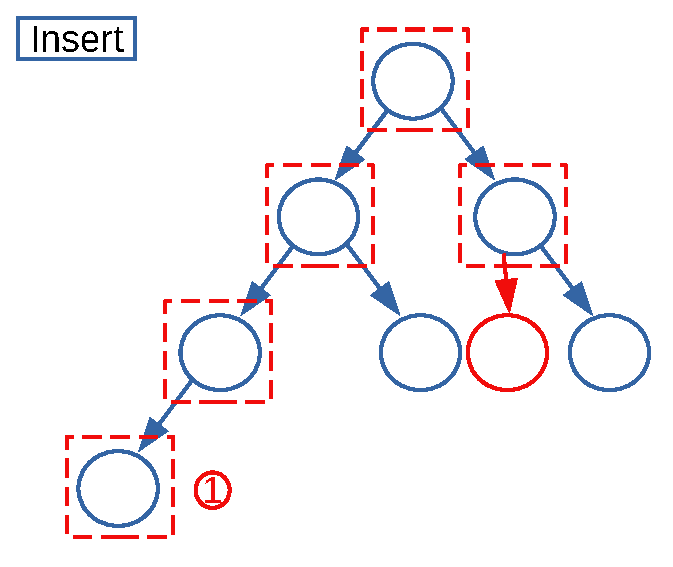
\includegraphics[scale=.6]{chapters/trees/images/trees_10.pdf}
		\caption[Add an element of a tree]{Add an element of a tree}
		\label{trees_10}
	\end{center}
\end{figure}

\subsection{Perfect binary tree}
A perfect binary tree is a binary tree in which all the nodes have two children except the leaf which do not have any children. In this case the following results are valid

\begin{figure}[H]
	\begin{center}
		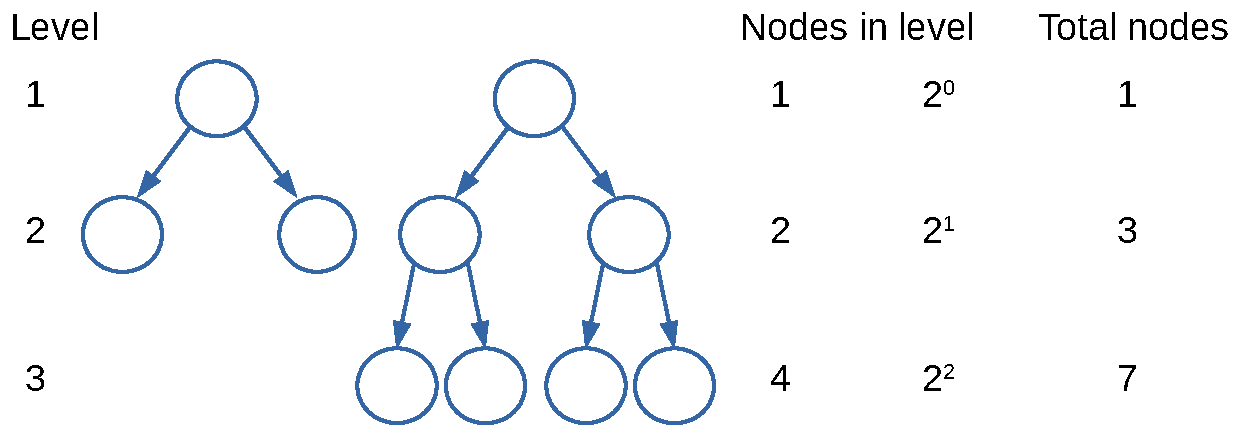
\includegraphics[scale=.6]{chapters/trees/images/trees_11.pdf}
		\caption[Perfect binary tree results]{Perfect binary tree results}
		\label{trees_11}
	\end{center}
\end{figure}

When a new row is added, the number of nodes double. Given a level \(n\) the total number of nodes is \(2n + 1\).